\section{Foster-Lyapunov Drift on Residue Quotients}

The phase-aware Lyapunov search turns the failed running-debt ansatz into a
more structured candidate.  Over \(100000\) sampled orbits in
\([10^6,10^9]\), the best grid point in
\[
  V(n;\alpha,\beta,\gamma_{\mathrm{diff}})
    = \log_2(n)+\alpha R(n)+\beta D_{\mathrm{running}}(n)
      + \text{phase offset}
\]
is \(\alpha=1.0\), \(\beta=0.0\), \(\gamma_{\mathrm{diff}}=0.0\), namely
\[
  V(n)=\log_2(n)+\vTwo(n+1).
\]
This reduces the same-sample V5 non-decrease fraction from
\(0.5001335415695829\) to \(0.1655372436648494\).  The tail-internal phase has
\(0.0\) non-decrease, and the remaining positive jumps are post-exit steps with
large \(R'=\vTwo(\Syr(n)+1)\) spikes
\(\artifact{phase_lyapunov_search.json}{phase\_lyapunov\_search.json}\).

The one-step Foster audit confirms the marginal drift but rejects uniform
one-step residue negativity.  Across the five windows
\([10^2,10^4]\) through \([10^{12},10^{15}]\), the marginal drift of \(V\) is
empirically consistent with \(\log_2(3/4)\): the deepest-window estimate is
\(-0.4123424992788405\) with CI
\[
  [-0.41856572879163634,\,-0.4061192697660446],
\]
and the saved one-step verdict is
\(\texttt{drift\_residue\_obstruction}\)
\(\artifact{phase_lyapunov_foster_drift.json}{phase\_lyapunov\_foster\_drift.json}\).

The obstruction is arithmetic rather than marginal.  At one step, residue
conditional drift fails uniform negativity for every tested
\(k\in\{3,4,5,6\}\), with \(50\) obstruction witnesses.  The visible cascade in
the first window \([10^2,10^4]\) is
\[
\begin{array}{rcl}
n\equiv 1 \pmod 8   &:& 0.5954199142013228,\quad
  \mathrm{CI}\ [0.5830610092394827,0.6077788191631629],\\
n\equiv 9 \pmod {16} &:& 1.5919631928192652,\quad
  \mathrm{CI}\ [1.5747431836625472,1.6091832019759833],\\
n\equiv 41 \pmod {64} &:& 3.557870295871902,\quad
  \mathrm{CI}\ [3.5249778818408877,3.5907627099029162].
\end{array}
\]
The same \(41\bmod 64\) class remains the largest obstruction across later
windows
\(\artifact{phase_lyapunov_foster_drift.json}{phase\_lyapunov\_foster\_drift.json}\).

\begin{figure}
  \centering
  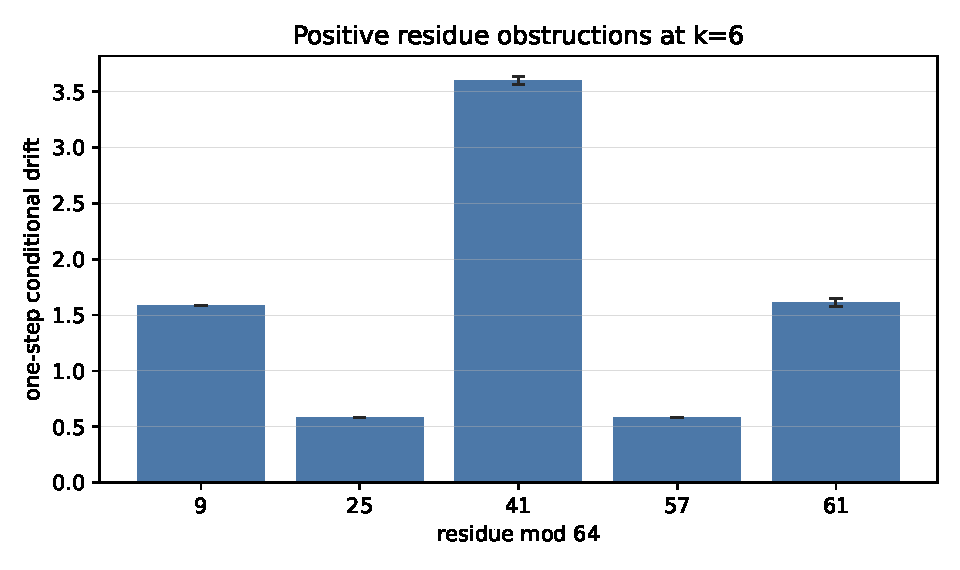
\includegraphics[width=0.86\linewidth]{figures/foster_residue_obstruction.pdf}
  \caption{Positive one-step residue obstructions at \(k=6\), regenerated from
  \artifact{phase_lyapunov_foster_drift.json}{phase\_lyapunov\_foster\_drift.json}.}
  \label{fig:foster-obstruction}
\end{figure}

The m-step audit closes this finite residue-Markov version of the question on
the tested grid.  For \(m\in\{1,2,4,8,16,32,64\}\), the smallest value with
residue-conditional drift uniformly negative across all tested windows and
residue powers is \(m=16\), and the same \(m=16\) also clears the
\(\epsilon=0.1\) margin.  At \(m=64\), the obstruction count is \(0\).  The
binding class before clearance is still \(n\equiv 41\pmod {64}\): it is the
maximal obstruction at \(m=1,2,4,8\), then disappears at \(m=16\)
\(\artifact{m_step_foster_drift.json}{m\_step\_foster\_drift.json}\).

\begin{figure}
  \centering
  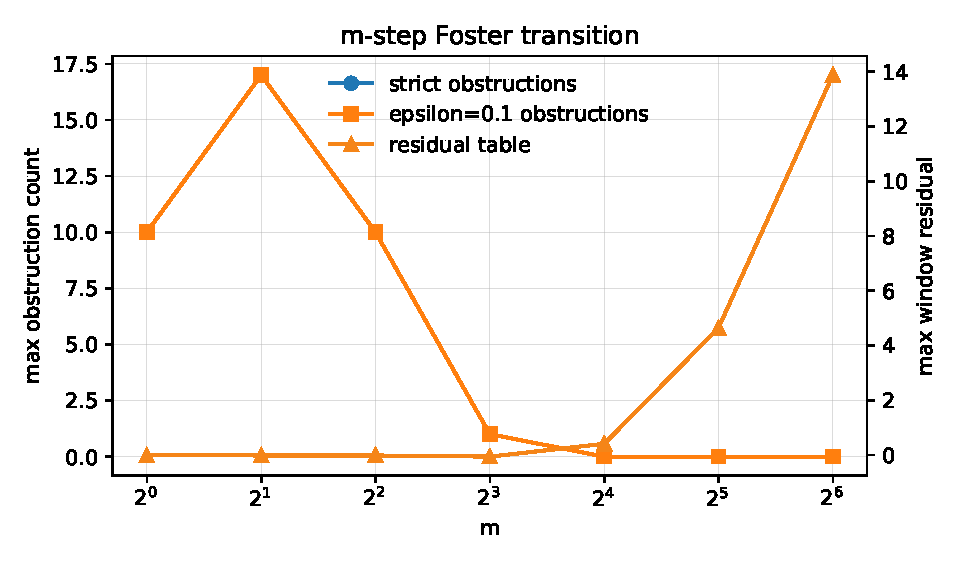
\includegraphics[width=0.86\linewidth]{figures/m_step_foster_transition.pdf}
  \caption{Transition from one-step obstruction to \(m\)-step residue-uniform
  negativity on the tested grid, regenerated from
  \artifact{m_step_foster_drift.json}{m\_step\_foster\_drift.json}.}
  \label{fig:mstep}
\end{figure}

The candidate Lyapunov satisfies the m-step Foster-Lyapunov drift condition
(Meyn-Tweedie, Markov Chains and Stochastic Stability, ch. 11) on residue
quotients mod \(2^k\) for \(k \in \{2,3,4,5,6\}\) at sample windows
\(n_0 \in [10^2, 10^{15}]\), with smallest tested grid value \(m = 16\) and
geometric-ergodicity margin \(\epsilon = 0.1\). The Collatz orbit is
deterministic, not a Markov chain; this is a finite empirical diagnostic on the
residue Markov chain quotient, not a theorem about deterministic per-orbit
descent.

This paragraph is deliberately close to the saved audit language
\(\artifact{m_step_foster_drift.json}{m\_step\_foster\_drift.json}\).  The
underlying Markov-chain reference is Meyn and Tweedie
\cite[Ch.~11]{meynTweedie2009}; the deterministic Collatz orbit is not itself a
Markov chain.
